\documentclass[11pt,letterpaper]{article}
\usepackage[utf8]{inputenc}
\usepackage[T1]{fontenc}
\usepackage{lmodern}
\usepackage[margin=1in]{geometry}
\usepackage{amsmath,amssymb,amsfonts,amsthm}
\usepackage{booktabs}
\usepackage{microtype}
\usepackage{enumitem}
\usepackage{fancyhdr}
\usepackage{titlesec}
\usepackage{xcolor}
\usepackage{tikz}
\usepackage{pgfplots}
\usepackage{mdframed}
\usepackage[hidelinks,colorlinks=true,linkcolor=SlateBlue,citecolor=SlateBlue,urlcolor=Terracotta]{hyperref}

\pgfplotsset{compat=1.18}
\usetikzlibrary{arrows.meta,positioning,calc,patterns,decorations.pathreplacing}

\definecolor{SlateBlue}{HTML}{1E293B}
\definecolor{Terracotta}{HTML}{C2410C}
\definecolor{ForestGreen}{HTML}{15803D}
\definecolor{LightSlate}{HTML}{F8FAFC}
\definecolor{BorderGray}{HTML}{CBD5E1}
\definecolor{LightTerracotta}{HTML}{FFF7ED}
\definecolor{CourseBlue}{HTML}{0072B2}
\definecolor{CourseOrange}{HTML}{D55E00}
\definecolor{CourseTeal}{HTML}{009E73}
\definecolor{CoursePurple}{HTML}{CC79A7}
\definecolor{CourseAmber}{HTML}{E69F00}

\titleformat{\section}{\normalfont\Large\bfseries\color{SlateBlue}}{\thesection}{1em}{}[\titlerule]
\titleformat{\subsection}{\normalfont\large\bfseries\color{SlateBlue}}{\thesubsection}{1em}{}
\titleformat{\subsubsection}{\normalfont\normalsize\bfseries\color{Terracotta}}{\thesubsubsection}{1em}{}

\pagestyle{fancy}
\fancyhf{}
\renewcommand{\headrulewidth}{0.4pt}
\renewcommand{\footrulewidth}{0.4pt}
\fancyhead[L]{\small\scshape\color{SlateBlue}\leftmark}
\fancyhead[R]{\small\color{SlateBlue}Principles of Economics}
\fancyfoot[C]{\thepage}

\newmdenv[
  linecolor=Terracotta,
  linewidth=1.5pt,
  backgroundcolor=LightTerracotta,
  innertopmargin=10pt,
  innerbottommargin=10pt,
  innerrightmargin=12pt,
  innerleftmargin=12pt,
  roundcorner=4pt,
  skipabove=12pt,
  skipbelow=12pt
]{coreprinciple}

\newmdenv[
  linecolor=SlateBlue,
  linewidth=1.5pt,
  backgroundcolor=LightSlate,
  innertopmargin=10pt,
  innerbottommargin=10pt,
  innerrightmargin=12pt,
  innerleftmargin=12pt,
  roundcorner=4pt,
  skipabove=12pt,
  skipbelow=12pt
]{casestudy}

\newenvironment{examplecase}[1]{%
  \begin{casestudy}
  \boxheader{SlateBlue}{#1}
  \vspace{0.4em}
}{%
  \end{casestudy}
}

\newmdenv[
  linecolor=BorderGray,
  linewidth=1pt,
  backgroundcolor=white,
  innertopmargin=10pt,
  innerbottommargin=10pt,
  innerrightmargin=12pt,
  innerleftmargin=12pt,
  roundcorner=4pt,
  skipabove=12pt,
  skipbelow=12pt
]{takeaways}

\newcommand{\boxheader}[2]{{\noindent\bfseries\color{#1}\Large #2}\vspace{0.4em}\par}

% ==============================================================================
% TikZ & PGFPlots Global Configuration and Economics Styling
% ==============================================================================

\usepackage{tikz}
\usepackage{pgfplots}
\pgfplotsset{compat=1.18}

% TikZ Libraries
\usetikzlibrary{
    arrows.meta,
    positioning,
    calc,
    shapes.geometric,
    patterns,
    decorations.pathreplacing,
    intersections
}

% Common Economics TikZ Styles
\tikzset{
    % Axes and Structural Lines
    econ axis/.style={->, >=Stealth, thick, color=SlateBlue!90!black},
    econ grid/.style={thin, dashed, color=gray!30},
    econ guide/.style={dashed, color=gray!60, thin},
    % Curves and Functions
    demand curve/.style={very thick, color=SlateBlue},
    supply curve/.style={very thick, color=Terracotta},
    mb curve/.style={very thick, color=SlateBlue},
    mc curve/.style={very thick, color=Terracotta},
    % Points and Highlights
    econ point/.style={circle, fill=SlateBlue!90!black, inner sep=1.8pt},
    econ highlight/.style={fill=Terracotta!20, opacity=0.5},
    % Annotations
    econ label/.style={font=\small\sffamily, align=center},
    econ annotation/.style={font=\footnotesize\itshape, color=SlateBlue!80!black}
}

% PGFPlots Standard Economics Style
\pgfplotsset{
    econ diagram/.style={
        axis lines=left,
        xlabel style={at={(ticklabel* cs:1)}, anchor=north west, font=\small\bfseries},
        ylabel style={at={(ticklabel* cs:1)}, anchor=south east, font=\small\bfseries},
        label style={font=\small},
        tick label style={font=\small},
        grid=none,
        enlargelimits=false,
        axis line style={->, >=Stealth, thick, color=SlateBlue!90!black}
    }
}

\usepackage{tcolorbox}

\begin{document}

\title{\Huge\bfseries\color{SlateBlue} Chapter 8: Aggregate Demand and Aggregate Supply (AD-AS)}
\author{\large Principles of Macroeconomics Curriculum}
\date{2026}
\maketitle

\thispagestyle{plain}

\begin{abstract}
This chapter provides a rigorous, pedagogical treatment of Chapter 8: Aggregate Demand and Aggregate Supply (AD-AS), benchmarked to standard principles curriculum.
\end{abstract}

\tableofcontents
\vspace{1.5em}
\hrule
\vspace{1.5em}

% -----------------------------------------------------------------------------
% Section 8.1: Aggregate Demand Mechanics and Slope Explanations
% -----------------------------------------------------------------------------
\section{Aggregate Demand Mechanics and Slope Explanations}

\subsection*{1. Conceptual Introduction}
While the Keynesian cross assumes a fixed price level, the \textbf{Aggregate Demand and Aggregate Supply (AD-AS)} model allows both real output ($Y$) and the broad price level ($P$) to vary simultaneously. **Aggregate Demand ($AD$)** represents total planned spending on domestic final goods and services at each general price level, holding monetary and fiscal policy constant:
\begin{equation}
AD = C + I + G + NX
\end{equation}

Why does the $AD$ curve slope downward? Unlike microeconomic demand curves (which slope down because consumers substitute toward cheaper relative goods), the downward slope of the aggregate demand curve is driven by three macroeconomic mechanisms:
\begin{itemize}
    \item \textbf{The Wealth Effect (Real Balances Effect):} When the price level rises, the real purchasing power of household nominal wealth (bank accounts, bonds) declines, making consumers feel poorer and reducing consumption spending ($C \downarrow$).
    \item \textbf{The Interest Rate Effect:} A higher price level increases money demand, driving up nominal and real interest rates. Higher borrowing costs discourage business investment and household mortgage borrowing ($I \downarrow$).
    \item \textbf{The Exchange Rate Effect:} Higher domestic prices make domestic goods more expensive relative to foreign goods, reducing net exports ($NX \downarrow$).
\end{itemize}

\subsection*{2. Visual Representation}
Figure~\ref{fig:ad_curve_derivation} illustrates the downward-sloping Aggregate Demand curve, showing how a rise in the price level from $P_1$ to $P_2$ contracts real output demanded from $Y_1$ to $Y_2$ through wealth, interest-rate, and exchange-rate channels.

\begin{tcolorbox}[colback=yellow!10!white,colframe=orange!80!black,title=\textbf{Clear It Up: Price Level Versus Aggregate Demand}]
A change in the economy's price level causes a \textbf{movement along} a stationary $AD$ curve. A change in consumer confidence, monetary policy, government spending, or foreign income shifts the \textbf{entire $AD$ curve}. Confusing the two turns an outcome of the model into a cause of its shift.
\end{tcolorbox}

\begin{figure}[htbp]
\centering
\begin{tikzpicture}[scale=1.05]
    % Axes
    \draw[->, thick] (0,0) -- (6.2,0) node[below] {Real Output / GDP ($Y$)};
    \draw[->, thick] (0,0) -- (0,5.2) node[left] {Price Level ($P$)};
    \node[below left] at (0,0) {$0$};

    % AD curve: P = 5 - 0.8Q -> (0,4.5) to (5.6,0)
    \draw[very thick, color=blue!80!black] (0.5,4.5) -- (5.6,0) node[right] {Aggregate Demand ($AD$)};

    % Price P1 (y = 3.2) -> Y1 = 2.25 (x=2.25)
    \draw[dashed] (0,3.2) node[left] {$P_1$} -- (2.25,3.2);
    \draw[dashed] (2.25,0) node[below] {$Y_1$} -- (2.25,3.2);
    \filldraw[blue!80!black] (2.25,3.2) circle (2.2pt);

    % Price P2 (y = 1.8) -> Y2 = 4.0 (x=4.0)
    \draw[dashed] (0,1.8) node[left] {$P_2$} -- (4.0,1.8);
    \draw[dashed] (4.0,0) node[below] {$Y_2$} -- (4.0,1.8);
    \filldraw[blue!80!black] (4.0,1.8) circle (2.2pt);

    % Arrow showing movement along AD
    \draw[->, thick, color=Terracotta] (2.4,3.0) -- node[above right, font=\scriptsize] {Wealth & Interest Rate Effects} (3.8,2.0);
\end{tikzpicture}
\caption{Downward Slope of Aggregate Demand. A higher price level ($P_1 \to P_2$) reduces real wealth and raises interest rates, causing a movement up and left along the $AD$ curve from $Y_2$ to $Y_1$.}
\label{fig:ad_curve_derivation}
\end{figure}

\subsection*{3. Real-World Application: Federal Reserve Interest Rate Hikes and Housing Demand}
When the Federal Reserve raises its policy rate to combat inflation, mortgage rates jump from $3\%$ to $7\%$. This interest rate effect discourages homebuilding and consumer durable goods purchases, shifting aggregate demand leftward and cooling inflationary pressures across the macroeconomy.

\subsection*{4. Mathematical Foundation (Algebra Level)}
A linear aggregate demand equation links real output demanded to the price level $P$ and autonomous spending shifts $A$:
\begin{equation}
Y^d = A - \lambda P, \qquad \text{where } \lambda > 0
\end{equation}

\noindent\textbf{Worked Problem:}
An economy's aggregate demand schedule is $Y^d = 3{,}000 - 400P$, where $Y$ is in billions of chained dollars and $P$ is the price level index (e.g., $P = 1.25$).
\begin{enumerate}
    \item Compute real output demanded when $P_1 = 1.00$ and when $P_2 = 1.25$.
    \item Suppose monetary policy easing adds $\$200\text{ billion}$ in autonomous spending at every price level, shifting $AD$ to $Y^d = 3{,}200 - 400P$. Compute the new output demanded at $P = 1.25$.
\end{enumerate}

\noindent\textbf{Step-by-Step Breakdown:}
\begin{enumerate}
    \item \textbf{Calculate Output Demanded at $P_1 = 1.00$ and $P_2 = 1.25$:}
    \[
    Y_1^d(1.00) = 3{,}000 - 400(1.00) = \mathbf{\$2{,}600\text{ billion}}
    \]
    \[
    Y_2^d(1.25) = 3{,}000 - 400(1.25) = 3{,}000 - 500 = \mathbf{\$2{,}500\text{ billion}}
    \]

    \item \textbf{Calculate New Output Demanded After the $AD$ Shift ($P = 1.25$):}
    \[
    Y^d_{\text{new}}(1.25) = 3{,}200 - 400(1.25) = 3{,}200 - 500 = \mathbf{\$2{,}700\text{ billion}}
    \]
\end{enumerate}
\textbf{Conclusion:} A price level increase from $1.00$ to $1.25$ reduces output demanded by $\$100\text{ billion}$, while monetary easing shifts the curve rightward, raising output demanded at $P = 1.25$ from $\$2{,}500\text{B}$ to $\$2{,}700\text{B}$.

% -----------------------------------------------------------------------------
% Section 8.2: Short-Run and Long-Run Aggregate Supply
% -----------------------------------------------------------------------------
\section{Short-Run and Long-Run Aggregate Supply}

\subsection*{1. Conceptual Introduction}
Aggregate supply describes the total quantity of goods and services firms produce and sell at each price level. Crucially, supply behavior differs sharply between the short run and the long run:
\begin{itemize}
    \item \textbf{Long-Run Aggregate Supply ($LRAS$):} In the long run, nominal wages and input prices fully adjust to price-level changes. Because productive capacity depends entirely on labor, capital, technology, and natural resources—not on the price level—the $LRAS$ curve is **vertical at Potential Output ($Y^*$)**.
    \item \textbf{Short-Run Aggregate Supply ($SRAS$):} In the short run, sticky nominal wages and sticky menu prices mean that an unexpected rise in the price level makes production temporarily more profitable, causing firms to expand output above potential ($Y > Y^*$). Consequently, the $SRAS$ curve slopes **upward**.
\end{itemize}

When aggregate demand intersects $SRAS$ and $LRAS$ simultaneously, the economy achieves **macroeconomic equilibrium**. If $AD$ shifts, the economy experiences either a recessionary gap ($Y < Y^*$, high unemployment) or an inflationary gap ($Y > Y^*$, overheating and rising inflation). Over time, flexible wage and price adjustments cause the $SRAS$ curve to shift, automatically steering the economy back to long-run potential output $Y^*$.

\subsection*{2. Visual Representation}
Figure~\ref{fig:adas_equilibrium} illustrates macroeconomic equilibrium at potential output $Y^*$, alongside recessionary and inflationary gap regions.

\begin{figure}[htbp]
\centering
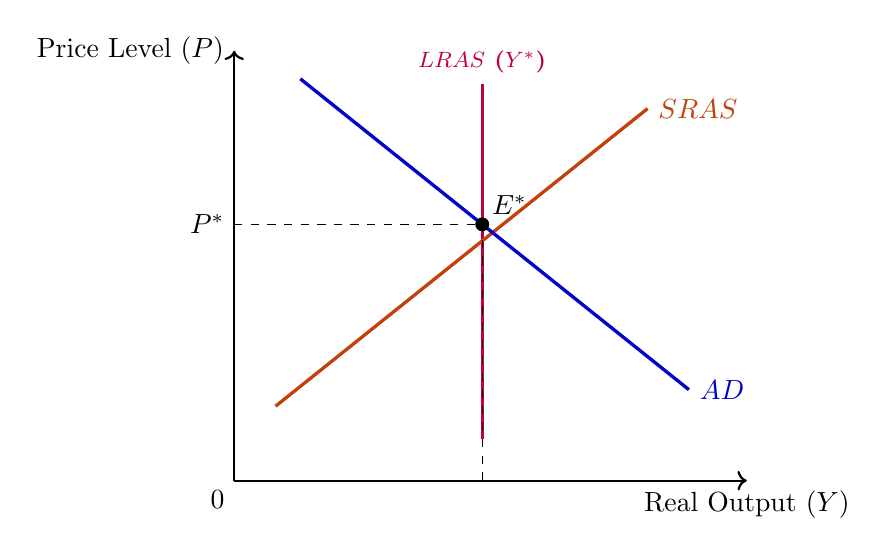
\begin{tikzpicture}[scale=1.05]
    % Axes
    \draw[->, thick] (0,0) -- (6.2,0) node[below] {Real Output ($Y$)};
    \draw[->, thick] (0,0) -- (0,5.2) node[left] {Price Level ($P$)};
    \node[below left] at (0,0) {$0$};

    % LRAS vertical at Y* (x = 3.0)
    \draw[very thick, color=purple] (3.0,0.5) -- (3.0,4.8) node[above, font=\footnotesize\bfseries] {$LRAS$ ($Y^*$)};

    % SRAS upward sloping: P = 0.5 + 0.8Q -> (0.5,0.9) to (5.0,4.5)
    \draw[very thick, color=Terracotta] (0.5,0.9) -- (5.0,4.5) node[right] {$SRAS$};

    % AD downward sloping: P = 5.5 - 0.8Q -> (0.8,4.86) to (5.5,1.1)
    \draw[very thick, color=blue!80!black] (0.8,4.86) -- (5.5,1.1) node[right] {$AD$};

    % Equilibrium E* at (3.0, 3.1)
    \draw[dashed] (0,3.1) node[left] {$P^*$} -- (3.0,3.1);
    \draw[dashed] (3.0,0) -- (3.0,3.1);
    \filldraw[black] (3.0,3.1) circle (2.2pt) node[above right] {$E^*$};
\end{tikzpicture}
\caption{Macroeconomic Equilibrium in AD-AS. Long-run equilibrium occurs where aggregate demand ($AD$), short-run aggregate supply ($SRAS$), and vertical long-run aggregate supply ($LRAS$) intersect at potential output $Y^*$ and price level $P^*$.}
\label{fig:adas_equilibrium}
\end{figure}

\subsection*{3. Real-World Application: Stagflation from Adverse Supply Shocks}
During the 1970s oil shocks, soaring crude oil prices shifted the $SRAS$ curve leftward—causing output to fall (recession) while the price level spiked (inflation). This painful combination of economic stagnation and inflation is called **stagflation**, which presents a severe dilemma for policymakers because fighting inflation worsens unemployment, while stimulating demand worsens inflation.

\subsection*{4. Mathematical Foundation (Algebra Level)}
Short-run aggregate supply is modeled as:
\begin{equation}
P = P^e + \gamma(Y - Y^*) + \rho
\end{equation}
where $P^e$ is expected price, $\gamma$ captures wage stickiness, and $\rho$ represents supply shocks (such as oil price spikes).

\noindent\textbf{Worked Problem:}
An economy has vertical long-run aggregate supply at $Y^* = \$10\text{ trillion}$, aggregate demand $AD: P = 3.0 - 0.1Y$, and short-run aggregate supply $SRAS: P = 0.5 + 0.15Y$.
\begin{enumerate}
    \item Compute short-run macroeconomic equilibrium $(Y_1^*, P_1^*)$.
    \item Identify whether the economy is in a recessionary or inflationary gap.
\end{enumerate}

\noindent\textbf{Step-by-Step Breakdown:}
\begin{enumerate}
    \item \textbf{Set $AD = SRAS$ and Solve for Short-Run Equilibrium ($Y_1^*, P_1^*$):}
    \[
    3.0 - 0.1Y_1^* = 0.5 + 0.15Y_1^* \implies 2.5 = 0.25Y_1^* \implies Y_1^* = \mathbf{\$10\text{ trillion}}
    \]
    Substitute $Y_1^* = 10$ into either equation:
    \[
    P_1^* = 3.0 - 0.1(10) = 3.0 - 1.0 = \mathbf{2.0}
    \]

    \item \textbf{Compare $Y_1^* = \$10\text{T}$ to Potential Output $Y^* = \$10\text{T}$:}
    Because $Y_1^* = Y^*$, the economy is in **long-run macroeconomic equilibrium** with zero output gap.
\end{enumerate}
\textbf{Conclusion:} The market clears precisely at potential output $Y^* = \$10\text{ trillion}$ and price level $P = 2.0$.

% -----------------------------------------------------------------------------
% Section 8.3: Demand Shocks, Supply Shocks, and Self-Correction
% -----------------------------------------------------------------------------
\section{Demand Shocks, Supply Shocks, and Self-Correction}

\subsection*{1. Conceptual Introduction}
When exogenous shocks hit the macroeconomy, the AD-AS model traces how the system adjusts over time:
\begin{itemize}
    \item \textbf{Demand Shocks:} A sudden drop in consumer confidence or export demand shifts $AD$ leftward, creating a recessionary gap ($Y < Y^*$). Over time, as unemployed workers accept lower nominal wage increases, the $SRAS$ curve shifts \textbf{rightward (downward)}, gradually restoring full-employment output $Y^*$ at a lower price level.
    \item \textbf{Supply Shocks:} An adverse supply shock (such as a global oil embargo) shifts $SRAS$ leftward, generating stagflation. If policymakers use fiscal stimulus to fight the recession, they risk entrenching higher inflation; if they do nothing, the economy eventually self-corrects as resource prices recede.
\end{itemize}

\subsection*{2. Visual Representation}
Figure~\ref{fig:ad_shock_adjustment} traces a negative demand shock shifting $AD_1 \to AD_2$ (recession at $E_2$), followed by medium-run wage adjustment shifting $SRAS_1 \to SRAS_2$ to restore long-run potential output at $E_3$.

\begin{figure}[htbp]
\centering
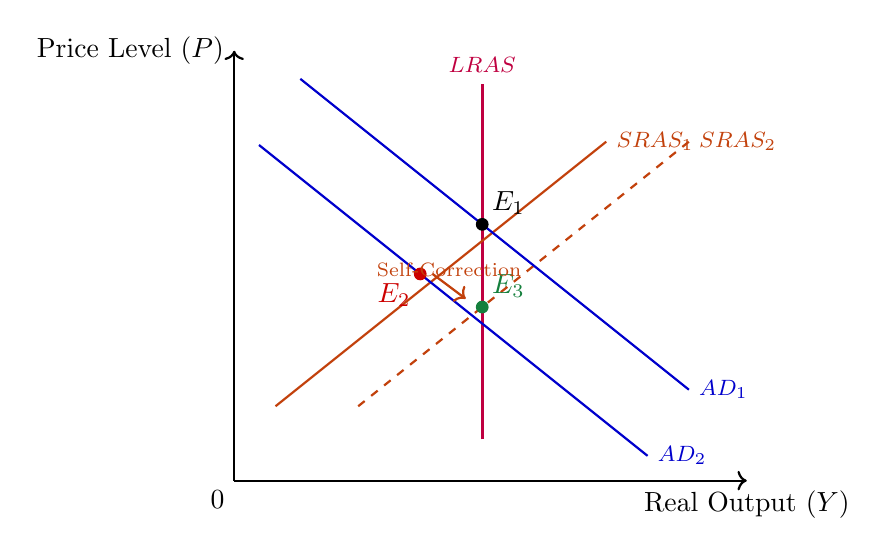
\begin{tikzpicture}[scale=1.05]
    % Axes
    \draw[->, thick] (0,0) -- (6.2,0) node[below] {Real Output ($Y$)};
    \draw[->, thick] (0,0) -- (0,5.2) node[left] {Price Level ($P$)};
    \node[below left] at (0,0) {$0$};

    % LRAS at Y* (x = 3.0)
    \draw[very thick, color=purple] (3.0,0.5) -- (3.0,4.8) node[above, font=\footnotesize] {$LRAS$};

    % SRAS1: P = 0.5 + 0.8Q -> (0.5,0.9) to (4.5,4.1)
    \draw[thick, color=Terracotta] (0.5,0.9) -- (4.5,4.1) node[right, font=\footnotesize] {$SRAS_1$};
    % SRAS2 (Downward shift): P = -0.3 + 0.8Q
    \draw[thick, dashed, color=Terracotta] (1.5,0.9) -- (5.5,4.1) node[right, font=\footnotesize] {$SRAS_2$};

    % AD1: P = 5.5 - 0.8Q -> (0.8,4.86) to (5.5,1.1)
    \draw[thick, color=blue!80!black] (0.8,4.86) -- (5.5,1.1) node[right, font=\footnotesize] {$AD_1$};
    % AD2 (Leftward shift): P = 4.3 - 0.8Q
    \draw[thick, color=blue!80!black] (0.3,4.06) -- (5.0,0.3) node[right, font=\footnotesize] {$AD_2$};

    % E1(3.0, 3.1) -> intersection of AD1 and SRAS1 on LRAS
    \filldraw[black] (3.0,3.1) circle (2pt) node[above right] {$E_1$};
    % E2(2.25, 2.5) -> recessionary intersection of AD2 and SRAS1
    \filldraw[red!80!black] (2.25,2.5) circle (2pt) node[below left] {$E_2$};
    % E3(3.0, 2.1) -> long-run self-corrected intersection of AD2 and SRAS2 on LRAS
    \filldraw[ForestGreen] (3.0,2.1) circle (2pt) node[above right] {$E_3$};

    \draw[->, thick, color=Terracotta] (2.4,2.5) -- node[above, font=\scriptsize] {Self-Correction} (2.8,2.2);
\end{tikzpicture}
\caption{Demand Shock and Macroeconomic Self-Correction. A negative demand shock shifts $AD_1 \to AD_2$, creating a recessionary gap at $E_2$. Over time, sticky wages adjust downward, shifting $SRAS_1 \to SRAS_2$ and restoring full employment at $E_3$.}
\label{fig:ad_shock_adjustment}
\end{figure}

\subsection*{3. Real-World Application: The 2020 Pandemic Shock and Policy Response}
In early 2020, government-mandated lockdowns caused a massive negative demand shock, shifting $AD$ leftward and driving U.S. unemployment to $14.7\%$. Unprecedented fiscal relief packages (`CARES Act`) injected trillions of dollars of transfer payments to shift $AD$ rapidly back rightward—preventing a prolonged depression-level self-correction process.

\subsection*{4. Mathematical Foundation (Algebra Level)}
Self-correction speed depends on the responsiveness of wage inflation to unemployment (the expectations-augmented Phillips Curve):
\begin{equation}
\pi_t = \pi_t^e - \beta(u_t - u_n) + \rho_t
\end{equation}

\noindent\textbf{Worked Problem:}
Starting from long-run equilibrium with $Y^* = \$10\text{T}$ and $P_1 = 2.0$, a drop in business optimism shifts aggregate demand leftward to $AD_2: P = 2.4 - 0.1Y$. If short-run aggregate supply remains fixed at $SRAS_1: P = 0.5 + 0.15Y$:
\begin{enumerate}
    \item Compute the short-run recessionary equilibrium $(Y_2^*, P_2^*)$ and output gap.
    \item Determine what price level must prevail in the medium run for $SRAS$ to self-correct back to $Y^* = \$10\text{T}$.
\end{enumerate}

\noindent\textbf{Step-by-Step Breakdown:}
\begin{enumerate}
    \item \textbf{Solve for Recessionary Equilibrium ($AD_2 = SRAS_1$):}
    \[
    2.4 - 0.1Y_2^* = 0.5 + 0.15Y_2^* \implies 1.9 = 0.25Y_2^* \implies Y_2^* = \mathbf{\$7.6\text{ trillion}}
    \]
    \[
    P_2^* = 2.4 - 0.1(7.6) = \mathbf{1.64}
    \]
    Output gap: $\frac{7.6 - 10.0}{10.0} \times 100\% = \mathbf{-24\%}$ (a severe recession).

    \item \textbf{Find Self-Corrected Price Level at $Y^* = \$10\text{T}$:}
    Substitute $Y = 10$ into the new $AD_2$ equation:
    \[
    P_{\text{new}} = 2.4 - 0.1(10) = \mathbf{1.40}
    \]
\end{enumerate}
\textbf{Conclusion:} The demand shock plunges output to $\$7.6\text{T}$ and price level to $1.64$. As wages adjust downward over time, the price level falls further to $1.40$ to restore full-employment potential output.

\end{document}